%% example.tex
%% Copyright (C) 2010,2011 Laura Dietz
%% Copyright (C) 2012 Jaakko Luttinen
%
% This work may be distributed and/or modified under the conditions of
% the LaTeX Project Public License, either version 1.3 of this license
% or (at your option) any later version.  The license is in the file
% LICENSE and the latest version of this license is in
% http://www.latex-project.org/lppl.txt and version 1.3 or later is
% part of all distributions of LaTeX version 2005/12/01 or later.
%
% This work has the LPPL maintenance status `maintained'.
% 
% The Current Maintainer of this work is Jaakko Luttinen.
%
% This work consists of the files bayesnet.sty and example.tex.

\documentclass[a4paper]{article}

%\usepackage{bayesnet}
\usepackage{tikz}
\usetikzlibrary{bayesnet}

\title{Graphical Models in Tikz}
\author{Laura Dietz, Jaakko Luttinen}

\begin{document}

\maketitle

TikZ examples for graphical models (Bayesian networks) and directed
factor graphs.

% A table of node types
\begin{table}[ht]
  \caption{Node types}
  \begin{center}
    \begin{tabular}{llc}
      Type & Syntax & Output
      \\
      \hline
      Latent variable &
      \texttt{\textbackslash node[latent]} &
      \tikz{\node[latent] {$x$};}
      \\
      Observed variable &
      \texttt{\textbackslash node[obs]} &
      \tikz{\node[obs] {$y$};}
      \\
      Constant &
      \texttt{\textbackslash node[const]} &
      \tikz{\node[const] {$a$};}
      \\
      Factor &
      \texttt{\textbackslash node[factor]} &
      \tikz{\node[factor] [label=$\mathcal{N}$] {}; }
      \\
      Plate &
      \texttt{\textbackslash plate} &
      \tikz{
        \node[latent] (x) {$x_m$};
        \newplate[x-plate] {(x)} {$m \in \mathcal{M}$};
      }
      \\
      Gate &
      &
      \tikz{
        % Nodes
        \node[latent] (l) at (0,3) {$\lambda$}; %
        \node[latent] (p) at (1.5,1.5) {$\phi$}; %
        \node[obs] (k) at (0,0) {$k$}; %
        % Factor
        % \nofactor {kf} {above=1 of k} {Multivariate} {above=1pt};
        \node[factor, label={[name=k-factor-caption]Multi}] (k-factor)
          at (0,1.5) {}; %
        % Gate
        \newgate[k-gate] {(k-factor)(k-factor-caption)} {l};
        % Connections
        \draw[<-] (k) -- (k-factor) edge[-] (p);
      }
    \end{tabular}
  \end{center}
\end{table}


% Simple Bayesian network
\begin{figure}[ht]
  \begin{center}
    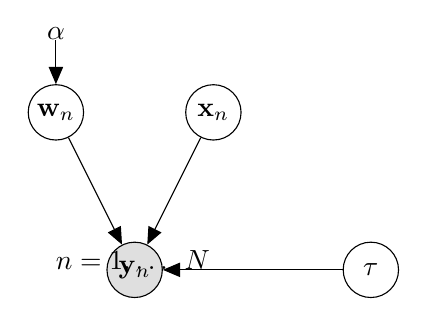
\begin{tikzpicture}
      % Define nodes
      \node[const]  (a) at (0,3) {$\alpha$};
      \node[latent] (w) at (0,2) {$\mathbf{w}_n$};
      \node[latent] (x) at (2,2) {$\mathbf{x}_n$};
      \node[latent] (t) at (4,0) {$\tau$};
      \node[obs]    (y) at (1,0) {$\mathbf{y}_n$};

      % Connect the nodes
      \draw[<-] (w) -- (a);
      \draw[<-] (y) edge (x)
                    edge (w)
                    edge (t);

      % Plates
      \newplate {(x)(y)(w)} {$n=1,\ldots,N$}
    \end{tikzpicture}
  \end{center}
  \caption{A simple Bayesian network.}
\end{figure}

% Latent Dirichlet allocation
\begin{figure}[ht]
  \begin{center}
    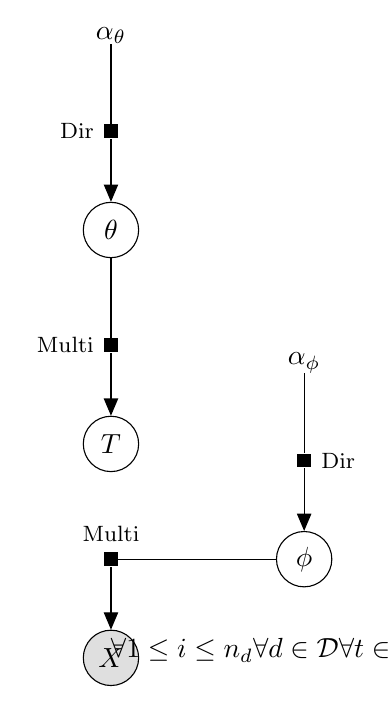
\begin{tikzpicture}[x=2cm,y=2cm]

      % Nodes

      \node[obs]                   (X)      {$X$} ; %
      \node[latent, above=of X]    (T)      {$T$} ; %
      \node[latent, above=of T]    (theta)  {$\theta$}; %
      \node[const, above=of theta] (atheta) {$\alpha_\theta$};


      % Factors
      \node[factor, above=of X, label={[name=X-factor-label]Multi}]
      (X-factor) {}; %
      \node[factor, above=of T, 
      label={[name=T-factor-label]left:Multi}] (T-factor) {}; %
      \node[factor, above=of theta,
      label={[name=theta-factor-label]left:Dir}] (theta-factor) {}; %

      % More nodes
      \node[latent, right=of X-factor] (phi) {$\phi$}; %
      \node[const, above=of phi]       (aphi) {$\alpha_\phi$}; %

      \node[factor, above=of phi, label={[name=phi-factor-label]right:Dir}]
      (phi-factor) {};

      \draw[<-] (X)     -- (X-factor)     edge[-] (phi);
      \draw[<-] (phi)   -- (phi-factor)   edge[-] (aphi);
      \draw[<-] (T)     -- (T-factor)     edge[-] (theta);
      \draw[<-] (theta) -- (theta-factor) edge[-] (atheta);

      \newgate[X-gate] {(X-factor)(X-factor-label)} {T}

      \newplate[plate1] {(X)(X-gate)(T)(T-factor)(T-factor-label)}
      {$\forall 1 \leq i \leq n_d$}; %
      \newplate {(plate1)(theta)(theta-factor)(theta-factor-label)}
      {$\forall d \in \mathcal{D}$} ; %
      \newplate {(phi)(phi-factor)(phi-factor-label)} {$\forall t \in
        \mathcal{T}$} ; %
      
    \end{tikzpicture}

  \end{center}

  \caption{Latent Dirichlet allocation as directed factor graph.}

\end{figure}

% Latent Dirichlet allocation
\begin{figure}[ht]
  \begin{center}
    \begin{tikzpicture}[x=2cm,y=2cm]
    \end{tikzpicture}
  \end{center}
\end{figure}


% Latent Dirichlet allocation
\begin{figure}[ht]
  \begin{center}
    \begin{tikzpicture}

      % Nodes
      
      \matrix[row sep=15pt,column sep=40pt, matrix anchor=mid] (lda) {
        &
        \\
        &
        \\
        \node (lambda) [latent] {$\theta$}; &
        \\
        \nofactor{drawtc}{}{Multi}{left=0pt}; &
        \\
        \node (tc) [latent] {$T$}; &
        \\
        \nofactor{drawxc}{}{Multi}{above=0pt}; \gate{gatexc}{(drawxc)
          (captdrawxc)}{$t$}; & \node (phi) [latent] {$\phi$};
        \\
        \node (xc) [obs] {$X$}; &
        \\
      };
      \nofactor{drawlambda}{above=15pt of lambda}{Dir}{right=0pt};
      \nofactor{drawphi}{above=15pt of phi}{Dir}{right=0pt};
      \node (alphalambda) [const, above=15pt of drawlambda]  {$\alpha_{\theta}$};
      \node (alphaphi) [const, above=15pt of drawphi]  {$\alpha_{\phi}$};

      % Connections
      
      \draw [->] (alphaphi) -- (drawphi) -- (phi);
      \draw [->] (alphalambda) -- (drawlambda) -- (lambda);
      \draw [->] (lambda) -- (drawtc) -- (tc);
      \draw [->] (phi) -- (drawxc) -- (xc);
      \draw [-*] (tc) -- (gatexc);

      % Plates

      \plate {contentplatec}
      {(tc)(xc)(drawtc)(drawxc)(captdrawtc)(captdrawxc)(gatexc)}
      {$\forall 1 \leq i \leq n_d $} {}

      \plate {userplatec}
      {(contentplatec)(lambda)(drawlambda)(captdrawlambda)} {$\forall
        d \in \mathcal{D}$} {}

      \plate {topicplate} {(phi)(drawphi)(captdrawphi)} {$\forall t
        \in \mathcal{T}$}{}

    \end{tikzpicture}

  \end{center}

  \caption{Latent Dirichlet allocation as directed factor graph.}

\end{figure}


\begin{figure}[h]
\begin{center}
% Citation Influence
\begin{tikzpicture}

\matrix[row sep=4mm,column sep=10mm, matrix anchor=mid] (citinf) {
&
&[3mm] \node (psi) [latent] {$\gamma$};
&[12mm,between origins] \node (balance) [latent] {$\lambda$};
&[12mm,between origins] \node (innov) [latent] {$\psi$};
\\

&
& \nofactor{drawf}{}{Multi}{left=0pt};
&\nofactor{drawbalance}{}{Bern}{left=0pt};
&
\\

\node (lambda) [latent] {$\theta$}; 
&
& \node (f) [latent]  {$C$}; 
&\node (s) [latent]  {$S$}; 
&
\\

\nofactor{drawtc}{}{Multi}{left=0pt};
&
& \nofactor{drawtd}{}{Multi}{above=0pt};\gate{gatetd}{(drawtd) (captdrawtd)}{$\mathcal{T}$};
&
&\nofactor{drawtdinnov}{}{Multi}{below=0pt};
\\

\node (tc) [latent]  {$T'$}; 
&
& \node (td) [latent]  {$T$}; 
&
&
\\

\nofactor{drawxc}{}{Multi}{above=0pt}; \gate{gatexc}{(drawxc) (captdrawxc)}{$t$};
&  \node (phi) [latent]  {$\phi$};
& \nofactor{drawxd}{}{Multi}{above=0pt}; \gate{gatexd}{(drawxd) (captdrawxd)}{$t$};
&
&
\\

\node (xc) [obs]  {$W'$}; 
&
&\node (xd) [obs]  {$W$}; 
&
&
\\
\\
};

\vertogate{gates}{(drawtd)(captdrawtd)}{$S=0$}{(drawtdinnov)(captdrawtdinnov)}{$S=1$};

\nofactor{drawlambda}{above=8pt of lambda}{Dir}{right=0pt};
\node (alphalambda) [const, above=10pt of drawlambda]  {$\alpha_{\theta}$};

\nofactor{drawphi}{above=8pt of phi}{Dir}{right=0pt};
\node (alphaphi) [const, above=10pt of drawphi]  {$\alpha_{\phi}$};

\nofactor{drawpsi}{above=8pt of psi}{Dir}{left=0pt};
\node (alphapsi) [const, above=18pt of drawpsi] {$\alpha_{\gamma}$}; 

\nofactor{drawbalancep}{above=8pt of balance}{Beta}{left=0pt};
\node (alphabalance1) [const, above left=18pt and 8 pt of drawbalancep] {$\alpha_{\lambda_{\theta}}$}; 
\node (alphabalance2) [const, above right=18pt and 8 pt of drawbalancep] {$\alpha_{\lambda_{\psi}}$}; 

\nofactor{drawinnovp}{above=8pt of innov}{Dir}{left=0pt};
\node (alphainnov) [const, above=18pt of drawinnovp] {$\alpha_{\psi}$}; 

\draw [->] (alphaphi) -- (drawphi) -- (phi);
\draw [->] (alphalambda) -- (drawlambda) -- (lambda);
\draw [->] (alphapsi) -- (drawpsi) -- (psi);
\draw [->] (alphabalance1) -- (drawbalancep) -- (balance);
\draw [-] (alphabalance2) -- (drawbalancep);
\draw [->] (alphainnov) -- (drawinnovp) -- (innov);

\draw [->] (psi) -- (drawf) -- (f);
\draw [->] (lambda) -- (drawtc) -- (tc);
\draw [->] (lambda) -- (drawtd) -- (td);
\draw [->] (phi) -- (drawxc) -- (xc);
\draw [->] (phi) -- (drawxd) -- (xd);
\draw [->] (balance) -- (drawbalance) -- (s);
\draw [->] (innov) -- (drawtdinnov) -- (td);


\draw [-*] (tc) -- (gatexc);
\draw [-*] (td) -- (gatexd);
\draw [-*] (f) -- (gatetd);
\draw [-*] (s) -- (gates);


\plate{contentplatec}{(tc)(xc)(drawtc)(drawxc)(captdrawtc)(captdrawxc)(gatexc)}{$\forall w' \in c$}{}
\plate{userplatec}{(contentplatec)(lambda)(drawlambda)(captdrawlambda)}{$\forall c \in \mathcal{C}$}{}
\plate{contentplated}{(f)(td)(xd)(drawtd)(drawxd)(drawf)(captdrawtd)(captdrawxd)(captdrawf)(gatetd)(gatexd)(gates)(s)(drawbalance)}{$\forall w \in d$}{}
\plate{userplated}{(contentplated)(psi)(drawpsi)(captdrawpsi)(balance)(drawbalance)(captdrawbalance)(innov)}{$\forall d \in \mathcal{D}$}{}

\plate{topicplate}{(phi)(drawphi)(captdrawphi)}{$\forall t \in \mathcal{T}$}{}


\end{tikzpicture}

\end{center}

\caption{Citation influence model with own topics as directed factor graph.\label{fig:Citinf-owntopics-model}}

\end{figure}

\end{document}
